% !TEX root = ../../../main.tex
% 来源：中学数学实验教材·第三册（高中数学）
% 章节：二次函数 / 二次函数
% 原始文件：5.tex，行 636-649
% 类型：tikz
% ---
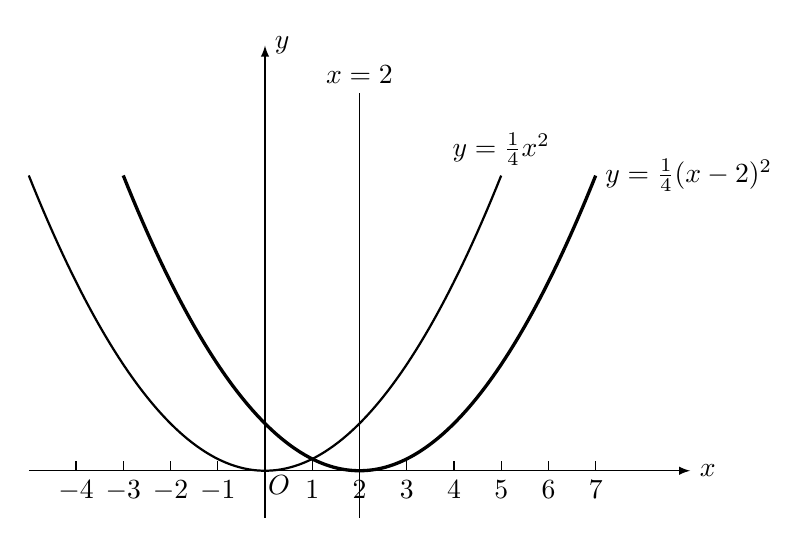
\begin{tikzpicture}[>=latex, scale=.6]
\draw[->] (-5,0)--(9,0)node[right]{$x$};
\draw[->] (0,-1)--(0,9)node[right]{$y$};
\foreach \x in {-4,-3,...,-1,1,2,...,7}
{
    \draw (\x,0)node[below]{$\x$}--(\x,.2);
}
\node at (.3,-.3){$O$};
\draw [domain=-5:5, samples=100, thick] plot(\x,{0.25*\x*\x});
\draw [domain=-3:7, samples=100, very thick] plot(\x,{0.25*(\x-2)*(\x-2)});
\draw (2,-1)--(2,8)node[above]{$x=2$};
\node at (5,6.25)[above]{$y=\frac{1}{4}x^2$};
\node at (7,6.25)[right]{$y=\frac{1}{4}(x-2)^2$};
\end{tikzpicture}
